\section{Confecção Ponte H}
A ponte H foi feita primeiramente em uma protoboard a fim de ser validada sua eficiência. Em seguida, o sistema foi transferido para a placa furada. O resistor utilizado apresentou mudança pois o item não estava disponível para a venda. Os resistores utilizados foram os 4 resistências de 560$\Omega$. Dessa forma:  

\begin{center}
	
	$\frac{3,3 - 0,7}{560}$ = $l_{b}$\\
	$l_{b}$ = 0,0046\textit{A}\\
	$I_{ce}$ = 1000 $\Omega$ * 0,0046 = 4,6 \textit{A}
	
\end{center}

\begin{itemize}

	\item $l_{b}$ = corrente que aciona o transistor;
	\item $I_{ce}$ = corrente disponível à carga.
	
\end{itemize}

O resultado final é mostrado a seguir:

\begin{figure}[H]
	\centering
	\includegraphics[width=13cm]{figuras/ponteHpronta.png}
	\caption{Ponte H confeccionada.}
	\label{ponte H pronta}
\end{figure}

Os integrantes que confeccionaram a placa tiveram dificuldades com a manipulação dos componentes, por não possuírem prática alguma com circuitos. Para posteriores trabalhos, é recomendado o uso de fios com bitolas maiores a fim de manter a segurança da ponte H.

\section{Confecção do plantário}

No sistema que está foi projetado para estufa, a área disponível para a locação da plantário era restrita a 50cmx50cm. Visto que esse espaço ainda seria compartilhado com os rolamentos da gaveta, a estrutura foi confeccionada em 3 tubos de PVC de 75mm de diâmetro e 40cm de comprimento. Além disso, foram feitos 2 furos em cada cano, com auxílio de serra-copo de 50mm de diâmetro, destinados a alocar as alfaces (as hortaliças do projeto). Os canos foram pintados de preto a fim de evitar o desenvolvimento de fungos e bactérias. O resultado é mostrado a seguir:

\begin{figure}[H]
	\centering
	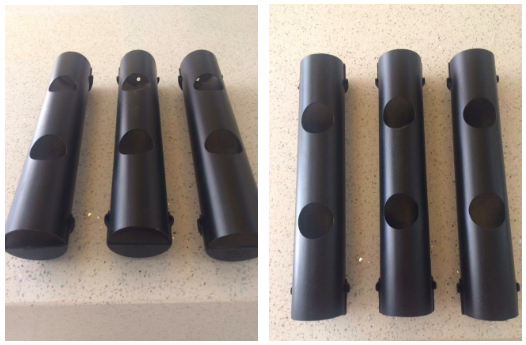
\includegraphics[width=13cm]{figuras/pvc.png}
	\caption{Plantário confeccionado com canos PVC. Fonte própria}
	\label{pvc}
\end{figure}

O sistema deve contar com uma bomba que eleve a água do reservatório para 40 cm acima do mesmo, onde estarão os canos. Os canos estarão dispostos com uma angulação que permite que o fluído percorra o cano pela ação da gravidade. Assim, não é preciso fazer cálculos de perdas de cargas das raízes do substrato. A potência pelo fluxo mássico é dado pela variação de energia na entrada e saída da bomba. Como representado a seguir, há a variação de energia de pressão, energia cinética e energia potencial:

\begin{center}
	${\displaystyle\frac{W}{m} = (\frac{P2}{\rho} + \frac{V2^2}{2} + gH2) - (\frac{P1}{\rho} + \frac{V1^2}{2} + gH1)}$	
\end{center}

Onde, 

$W$ = potência consumida (W/s);

$m$ = fluxo mássico (kg/s);

$P2$ = pressão no ponto 2;

$\rho$ = massa específica da água (kg/m³);

$V2$ = velocidade no ponto 2 (m/s)

$H2$ = altura no ponto 2 (m);

$g$ = gravidade (m²/s);

$P1$ = pressão no ponto 1;

$V1$ = velocidade no ponto 1 (m/s);

$H1$ = altura no ponto 1 (m);

Considera-se que não há variação de altura considerável entre a entrada e saída da bomba. Assim, não há variação de energia potencial. Considera-se também que não há variação de energia cinética no sistema (V2 aproximadamente igual a V1). Nota-se, então, que o sistema fornecerá apenas energia de pressão, essa mesma que torna possível a elevação da coluna de água. Dessa forma:

\begin{center}
	\large
	${\displaystyle \frac{W}{m} = H_g + \frac{P2-P1}{\rho}+ \frac{\Delta_p}{\rho g}}$
\end{center}

A variação de energia de pressão é dada por: 

\begin{center}
	\large
	${\displaystyle \Delta P = f \frac{L}{D} \frac{1}{2} \frac{Q^2}{A^2} \rho}$
\end{center}

Onde,

$f$ = fator de atrito;

$L$ = comprimento do escoamento (m) ;

$D$ = diâmetro;

$\rho$ = massa específica da água (kg/m³);

$A$ = área do escoamento ($m^2$);

$Q$ = vazão volumétrica ($m^3$/s).

Ao dividir a equação pela massa específica e gravidade, tem-se a altura manométrica (m):

\begin{center}
	\large
	${\displaystyle \Delta H = f \frac{L}{D} \frac{1}{2} \frac{Q^2}{A^2} \frac{1}{g}}$
\end{center}

É possível calculá-lo também a partir da equação de Coolebroke - White (1939). O fator de atrito de alguns materiais já são tabelados. A tabela a seguir dispõe de alguns dele:

\begin{figure}[H]
	\centering
	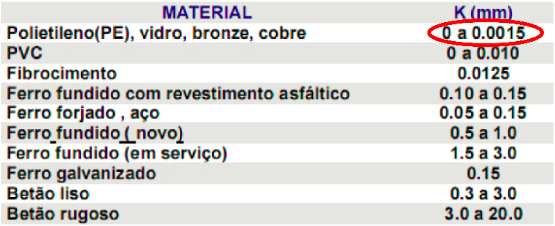
\includegraphics[width=13cm]{figuras/fatores_atrito.png}
	\caption{Fatores de atrito tabelados. Fonte: www.pipelife.com}
	\label{fatores_atrito}
\end{figure}

O material da tubulação de escoamento selecionada foi o polietileno, cujo fator de atrito é de 0,0015mm. O diâmetro do tubo é de 0,005m. A imagem a seguir o reporta já conectado aos tubos. 

\begin{figure}[H]
	\centering
	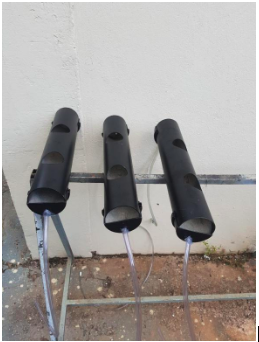
\includegraphics[width=8cm]{figuras/tubos_plantario.png}
	\caption{Tubos do plantário. Fonte própria}
	\label{fatores_atrito}
\end{figure}

Assim:

\begin{center}
	\large
	${\displaystyle \Delta H = 0,0015 \frac{0,7}{0,005} \frac{1}{2} \frac{3,33*10^-5}{\Pi^2 * (0,005)^4}}=302,01P_a$
\end{center}

\begin{center}
	\large
	${\displaystyle \Delta_h = \frac{\Delta_p}{\rho g} =0,03m}$
\end{center}
	
Onde, $\Delta_h$ é a perda de carga em metros.

Por fim, considera-se que a variação de pressão é dada por:

\begin{center}
	\large
	${\displaystyle P2 - P1= \rho g H}$
\end{center}


Dessa forma, têm-se:

\begin{center}
	\large
	${\displaystyle W= m(2gH + \frac{\Delta_p}{\rho g})= 0,274W}$
\end{center}



Como a perda de pressão distribuída é muito pequena em relação a altura e as especificações de bomba de aquário (solução) são vazão volumétrica e altura manométrica, a bomba ideal para o sistema fornece 120L/h e eleva 4,03m. Cada fornecedor de bombas trabalha com um rendimento específico do seu produto. O fornecedor de bomba Sarlobetter®, por exemplo, traz a curva característica de seus produtos. Nota-se que, para trabalhar na vazão encontrada. A bomba ideal é a S300 (300L/h) visto que com o aumento da coluna a ser vencida, a vazão decai e a bomba deixa de operar com sua vazão de projeto.  
Percebe-se que o cálculo da potência da bomba não envolveu rendimentos que variam de acordo com cada fabricante.
 

\begin{figure}[H]
	\centering
	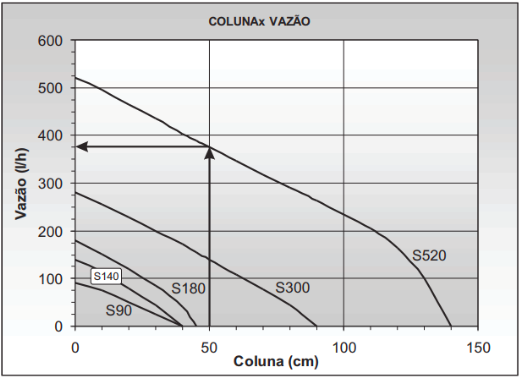
\includegraphics[width=13cm]{figuras/coluna.png}
	\caption{Curva característica da moto bomba Sarlo}
	\label{coluna}
\end{figure}

A fim de reduzir os custos, serão utilizadas bombas que os integrantes já possuíam. A primeira bomba é de 160L/h e 3,8W e a segunda de 240L/h e 4W, que já foram devidamente testadas. A terceira será comprada após a instalação das outras duas no sistema. A imagem a seguir retratada as duas bombas:

\begin{figure}[H]
	\centering
	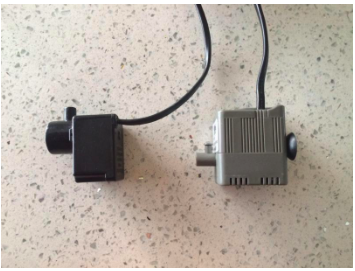
\includegraphics[width=8cm]{figuras/bombas.png}
	\caption{C Bombas de água. Fonte própria.}
	\label{coluna}
\end{figure}

O reservatório deverá conter também um compressor de ar com a finalidade de auxiliar no processo de dissolução dos nutrientes. Como seu fim é apenas mixer, sua seleção foi feita a partir do menor preço de mercado. O compressor que será utilizado é mostrado a seguir:

\begin{figure}[H]
	\centering
	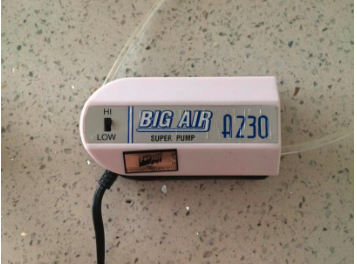
\includegraphics[width=8cm]{figuras/compressor.png}
	\caption{Compressor de ar. Fonte própria.}
	\label{compressor}
\end{figure}


\subsection{Confecção da ventilação}

Os coolers já foram instaladas na estrutura, na parte superior e em sentidos opostos, a fim de garantir a circulação de fluído no interior e para fora.

\begin{figure}[H]
	\centering
	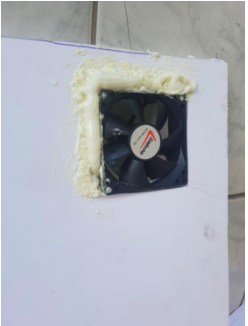
\includegraphics[width=8cm]{figuras/ventilador.png}
	\caption{Ventilador instalado na estrutura. Fonte própria.}
	\label{ventilador}
\end{figure}

O volume total do ambiente interno da estufa é dado por:

\begin{center}
	\large
	${\displaystyle V = b^2 * h = (0,5^2) * 0,7 = 0,175 m^3}$
\end{center}

Onde,

$V$ = volume total (m³);

$b$ = aresta da base quadrada (m);

$h$ = altura (m)

Dessa forma, o primeiro ventilador recicla esse mesmo volume em aproximadamente 16 segundos e o segundo o faz em aproximadamente 9 segundos.  

\section{Confecção iluminação}

Primeiramente foi implementado um parâmetro simples de W/área no qual o indicado para culturas como alface em hidroponia é de 40W/ft , porém devido a intensificação das pesquisas os parâmetros que possibilita melhores resultados são  PAR,PPF \& PPFD onde se utiliza valores diretamente associados ao processo de fotossíntese e fatores fisiológicos da planta.
A escolha entre as tecnologias HPS e LED foi a favor da escolha do LED devido a 3 fatores.

\textbf{1. Consumo de energia}

Consumo é um dos fatores mais importantes para o uso das lâmpadas de cultivo, o que fez as LEDs se tornarem a opção escolhida pois consomem menos energia que as HPS. consomem aproximadamente 90\% menos energia que as HPS.

\textbf{2. Vida útil}

Em comparação com lâmpadas HPS, a LED tem uma vida útil muito maior. Com o tempo as HQS podem se tornar mais fracas e perder a eficiência, ou seja, o custo real de funcionamento de uma HPS vai aumentando com seu uso.

\textbf{3. Calor gerado}

Para lâmpadas para cultivo indoor, as HPS emanam mais calor do que as luzes LED. O calor que as lâmpadas HPS produzem pode-se fazer necessário a compra de mais equipamentos de exaustão e ventilação, o que acaba gerando custos adicionais.

Levando como base estudos voltados a plantação hidropônica indoor, em especial os que a fonte luminosa fica próxima a planta , foi decidido o uso do modelo RBW(Red,Blue,White) em LED, no qual se utiliza led nas cores Vermelho, Azul e Branco por períodos de 16 horas de luz  nos quais os resultados demonstram melhores desempenhos das amostras plantadas. 

\begin{center}
	“As características sensoriais comercializáveis (crocância, doçura, forma e cor) de plantas frescas também foram avaliadas. As plantas foram cultivadas hidroponicamente com um fotoperíodo de 16 h a 24/20 ° C (dia / noite), 75 \% de umidade relativa, 900 $\mu$ mol mol -- 1 nível de CO2 e 210 $\mu$ mol m--2 s--1 densidade de fluxo de fótons sob RB LED , RGB e LED branco (RBW), e uma lâmpada fluorescente (FL, como controle) dentro de câmaras de crescimento por 20 dias (15 dias após a semeadura). ”
	
\end{center}
\begin{center}
 mol m--2 s--1 densidade de fluxo de fótons sob RB LED , RGB e LED branco (RBW), e uma lâmpada fluorescente (FL, como controle) dentro de câmaras de crescimento por 20 dias (15 dias após a semeadura). ”
 
\end{center}

Trechos retirados de artigos da Scientia Horticulturae  international journal.

Equipamento utilizado:

\begin{itemize}
	\item 1XLED full spectrum 28W 
	\item 2x LED Branco 3k 9W.
\end{itemize}

Com objetivo inicial de atender o parâmetro de 40W/ft e o máximo de simetria luminosa no projeto.

\begin{figure}[H]
	\centering
	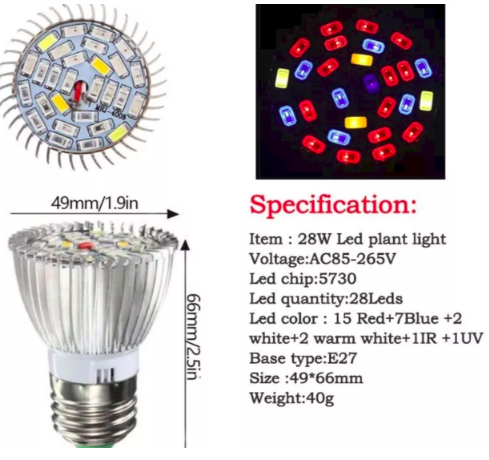
\includegraphics[width=8cm]{figuras/lampada_full.png}
	\caption{Lâmpada full spectrum}
	\label{lampada_full}
\end{figure}

\begin{figure}[H]
	\centering
	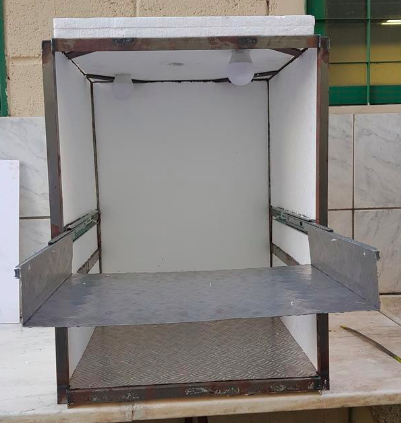
\includegraphics[width=8cm]{figuras/montagem.png}
	\caption{Montagem}
	\label{montagem}
\end{figure}

\begin{figure}[H]
	\centering
	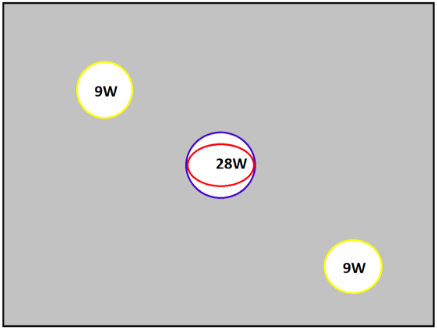
\includegraphics[width=8cm]{figuras/posicao_luminarias.png}
	\caption{Posição luminárias}
	\label{posicao_luminarias}
\end{figure}

A iluminação das lâmpadas com bulbo tem como projeção luminosa uma curva cardióide na qual a densidade luminosa no plano pode ser verificada no gráfico feito em Matlab.

\begin{figure}[H]
	\centering
	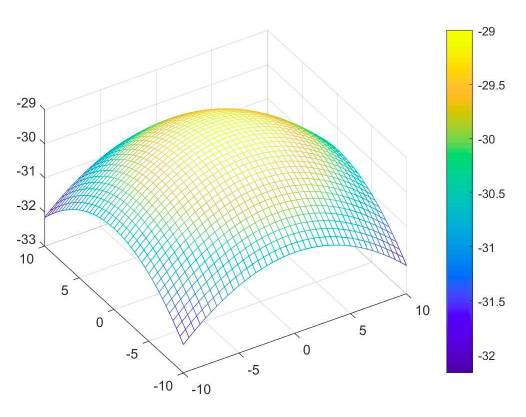
\includegraphics[width=8cm]{figuras/bulbo.png}
	\caption{Lâmpada BULBO}
	\label{bulbo}
\end{figure}

\section{Confecção Fonte}
Os Consumos que serão exigidos pelo projeto são:  

\textbf{5V:}

\begin{table}[H]
	\centering
	\begin{tabular}{|l|l|}
		\hline
		\multicolumn{1}{|c|}{PN} & \multicolumn{1}{c|}{Corrente(mA)} \\ \hline
		\multicolumn{1}{|c|}{PI 3} & \multicolumn{1}{c|}{2500} \\ \hline
		\multicolumn{1}{|c|}{sensor PH} & \multicolumn{1}{c|}{10} \\ \hline
		\multicolumn{1}{|c|}{PCF8591} &   \multicolumn{1}{c|}{50} \\ \hline
		\multicolumn{1}{|c|}{Total}&\multicolumn{1}{c|}{2560} \\ \hline
	\end{tabular}
	\caption{Consumo no projeto 5V}
	\label{Consumo no projeto 5V}
\end{table} 

\textbf{12V:}

\begin{table}[H]
	\centering
	\begin{tabular}{|l|l|}
		\hline
		\multicolumn{1}{|c|}{PN} & \multicolumn{1}{c|}{Corrente(mA)} \\ \hline
		\multicolumn{1}{|c|}{Motor DC} & \multicolumn{1}{c|}{2000} \\ \hline
		\multicolumn{1}{|c|}{FAN 12cm} & \multicolumn{1}{c|}{120} \\ \hline
		\multicolumn{1}{|c|}{FAN 8cm} &   \multicolumn{1}{c|}{80} \\ \hline
		\multicolumn{1}{|c|}{Total}&\multicolumn{1}{c|}{2200} \\ \hline
	\end{tabular}
	\caption{Consumo no projeto 12V}
	\label{Consumo no projeto 12V}
\end{table} 

Foi utilizado o software Proteus para o desenho do esquemático da fonte de 12V.


\begin{figure}[H]
	\centering
	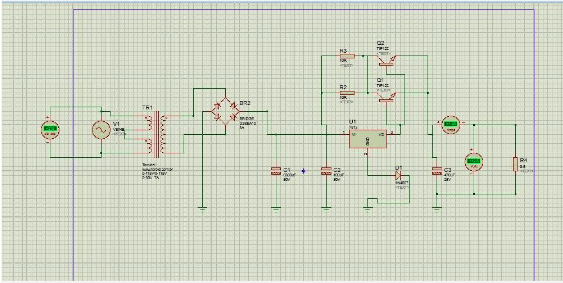
\includegraphics[width=15cm]{figuras/circuito_fonte_feita.png}
	\caption{Esquemático do circuito da fonte feito usando o software Proteus}
	\label{Circuito fonte feita}
\end{figure}

\begin{figure}[H]
	\centering
	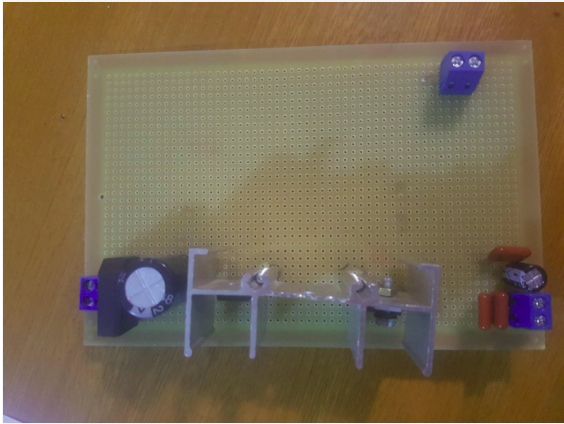
\includegraphics[width=10cm]{figuras/fonte_frente.png}
	\caption{Fonte pronta, parte de cima}
	\label{Fonte pronta parte de cima}
\end{figure}

\begin{figure}[H]
	\centering
	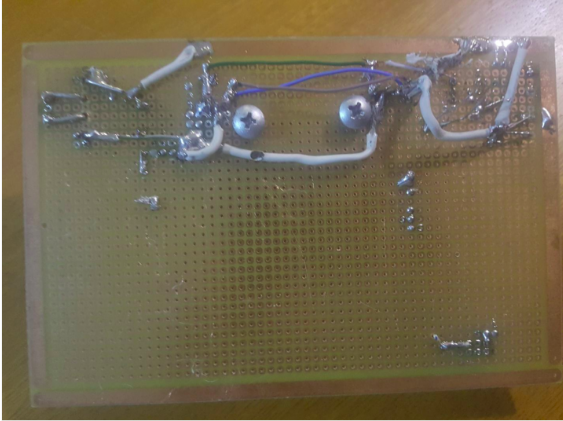
\includegraphics[width=10cm]{figuras/fonte_tras.png}
	\caption{Fonte pronta, parte de baixo}
	\label{Fonte pronta parte de trás}
\end{figure}


Os seguintes componentes foram utilizados  no projeto da fonte:

\begin{itemize}
	
	\item \textbf{TR4 (transformador):}   Tem como função abaixar a tensão de entrada AC oriunda da rede (240 Vrms) para um valor de tensão AC com amplitude de 20Vp.  
	
	\item \textbf{BR2 (Ponte retificadora)} Dispositivo eletrônico que tem como função transformar corrente alternada em corrente contínua.
	
\end{itemize}


\begin{figure}[H]
	\centering
	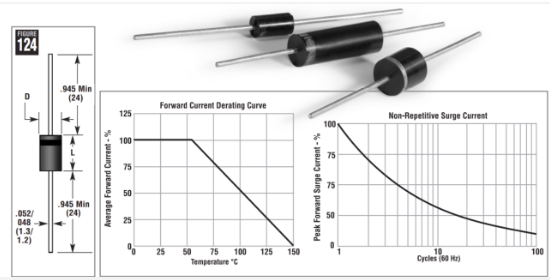
\includegraphics[width=10cm]{figuras/ponte_diodo.png}
	\caption{BR2 Ponte diodo}
	\label{Ponte diodo}
\end{figure}

\begin{itemize}
	\item \textbf{Capacitores de desacoplamento:} utilizados para manter a tensão estável após a retificação da onda.
	$V_{pp}$=40v→V secundário=20
\end{itemize}

\begin{center}
	$V_{pk}$ = $\sqrt{2}$ . $V_{AC}$ \\
	$V_{pk}$ = $\sqrt{2}$ . 20 \\
	Tensão  $V_{pk}$ = 28,3V \\
	f($V_{pk}$ 2 – VC min2) \\
	60(28.32+182)= C = 249,53$\mu$F \\
\end{center}

Dessa forma foi utilizado capacitor de 35v de 330$\mu$F.

\begin{itemize}
	\item \textbf{Regulador de Tensão 7812:} regulador linear de tensão, utilizado para polarizar a base dos  transistores.
	\item \textbf{R2 e R3:} usado limitar a corrente no coletor dos transistores.
	\item \textbf{C3:} capacitor de desacoplamento na saída.
	\item \textbf{Saída:} saída de 12v.

\end{itemize}

As medições foram feitas somente por multímetro por ser um projeto intermediário, entretanto medições finais serão analisadas por osciloscópio no qual é possível analisar a forma da onda final da fonte o que pode atestar melhor a qualidade.

Apesar de bem sucedida, foi determinado como objetivo  o melhoramento da fonte de energia construindo uma fonte chaveada na qual tem eficiência em torno de 80\% e utilizar como medição padrão das ondas de saída por um equipamento  osciloscópio ao invés de multímetro para verificar o desacoplamento e suavização do ripple no caso da fonte chaveada, dessa forma obtendo mais confiabilidade nos dados finais obtidos.
